\documentclass{article}
\usepackage{graphicx}
\usepackage{fullpage}
\usepackage{color}
\usepackage{listings}
\lstset{
basicstyle=\ttfamily,
language=C++,
%frame=single,
captionpos=b,
tabsize=2,
keywordstyle=\color{blue},
stringstyle=\color{mauve},
breaklines=true,
escapeinside={\%*}{*},
showspaces=false,
showstringspaces=false
}

\begin{document}
\title{Design of Pointer Memory Objects}
\date{}
\maketitle
\section{Motivation}
Consider the following simple program involving pointer dereferencing expressions.
\lstset{
caption=Motivating Example,
label=code:mot-example
}
\begin{lstlisting}
void fun()
{
  int val, *p, **q;
  p = &val;
  q = &p;
  *p = 10;
  **q = **q + 1;
}
\end{lstlisting}
%Let us assume the following sequence of analyses are run under the compositional framework (i) Points-to Analysis (ii) Constant Propagation Analysis. The points-to analysis has the %necessary information in the form of points-to graph[\ref{fig:ptg-example1}]. With this information it is possible to infer that the expressions \texttt{*p, **q} correspond to memory object %for the scalar variable \texttt{val} in Listing \ref{code:mot-example}
%\begin{figure}[h]
%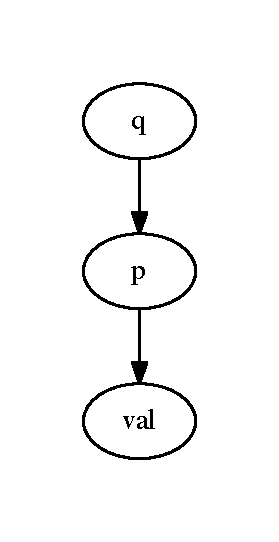
\includegraphics[scale=0.5]{ptg-example1.pdf}
%\caption{Points-to Graph for Motivating Example}
%\label{fig:ptg-example1}
%\end{figure}

\noindent To perform constant propagation analysis on the piece of code in Listing \ref{code:mot-example}, the analysis writer needs to write the transfer function for the $=$ operator (SgAssignOp) in which the state on rhs is transferred to the state on the lhs. See Section \ref{sec:sem-of-eq-op} for the semantics of the equals operator. Listing \ref{code:transfer-eq} shows a partial implementation of the transfer function. In general the client (constant propagation analysis) requests the composer for memory objects corresponding to parts it may encounter in its transfer functions. Similar to our example in Listing \ref{code:mot-example}, the dereferencing expression on the lhs of the $=$ operator can be arbitrarily complex, sometimes involving arrays. The default implementation (Syntax Analysis) returns PointerExprObject and ArrayExprObject for expressions involving pointers and arrays respectively. In this example, setting the state for PointerExprObj is incorrect since it does not correspond to the actual memory location. The framework however supports getDereference() method for Pointer/Array based objects. The semantics of the getDereference() method is to return the object pointed to by the corresponding pointer/array expression. The analysis writer is burdened with interpreting the sub-expressions using only the getDereference() to get the correct memory object. The transfer functions of the client analysis are left with no choice but to manipulate these arbitrary sub-expressions involving dereferencing operations.

\lstset{
label=code:transfer-eq,
caption=Transfer Function for Equals Operator
}
\begin{lstlisting}
void visit(SgAssignOp* sgn)
{
  MemLocObjectPtrPair lhsMem = composer->Expr2MemLoc(sgn->lhs_operand());
  MemLocObjectPtrPair rhsMem = composer->Expr2MemLoc(rhs->rhs_operand());
  // Get Lattices for the lhsMem, rhsMem, '=' operator
  // Copy the state from rhs to lhs and to the '=' operator
}
\end{lstlisting}

\noindent Instead of the getDereference() method, a cleaner API should handle Pointer/Array dereferencing expressions similar to variable references and the composer/server analysis should be responsible for returning the appropriate memory object.

\section{Semantics of Equals Operator}
\label{sec:sem-of-eq-op}

\end{document}